\documentclass[11pt]{article}
\usepackage[a4paper,margin=1in]{geometry}
\usepackage{graphicx}
\usepackage{amsmath}
\usepackage{subcaption}
\usepackage[T1]{fontenc}
\usepackage{lmodern}
\usepackage[utf8]{inputenc}
\usepackage{float}
\usepackage{hyperref}

\title{Comp 480/580 - Assignment \#2}
\author{Dev Sanghvi - \texttt{ds221}}
\date{Rice University \\ Date: 10/13/2025}

\begin{document}
\maketitle

\section*{Problem Overview}
This assignment compares three streaming sketch data structures, Count-Min, Count-Median, and Count-Sketch, on the heavy-hitter problem using the AOL query log. Words are tokenized from the \texttt{Query} column, inserted with unit weight into each sketch and into an exact dictionary, and then evaluated across multiple accuracy regimes. Our MurmurHash-based hash family uses $d=5$ rows and range $R\in\{2^{10},2^{14},2^{18}\}$ to produce pairwise-independent indices (and $\pm1$ signs for Count-Sketch).

\section{Implementation Summary}
\begin{itemize}
  \item \textbf{Driver}: streams tokens from disk, updates all sketches, and maintains an exact dictionary for evaluation.
  \item \textbf{Sketches}: Count-Min, Count-Median, and Count-Sketch share a common hashing interface; each supports \texttt{update()} and \texttt{estimate()}.
  \item \textbf{Top-$k$ tracker}: a min-heap maintains the best 500 tokens per sketch during streaming.
  \item \textbf{Outputs}: for each $R$, we produce error curves on three buckets (Frequent-100, Random-100, Infrequent-100) and a plot of the intersection size $|\text{Top-500}_\text{sketch}\cap\text{Top-100}_\text{truth}|$ versus $R$.
\end{itemize}

\section{Run Configuration}
All runs fix the random seed to ensure reproducibility. We use $d=5$ and $R\in\{2^{10},2^{14},2^{18}\}$ as required. The dataset is processed in a single pass. The exact dictionary's space usage is recorded and noted in the analysis.

\section{Plots}
Figures~\ref{fig:error-r1024}--\ref{fig:error-r262144} show the relative-error profiles for each sketch at each $R$, and Figure~\ref{fig:top500} reports the required top-500 intersection across $R$.

\begin{figure}[H]
  \centering
  \begin{subfigure}[t]{0.32\linewidth}
    \centering
    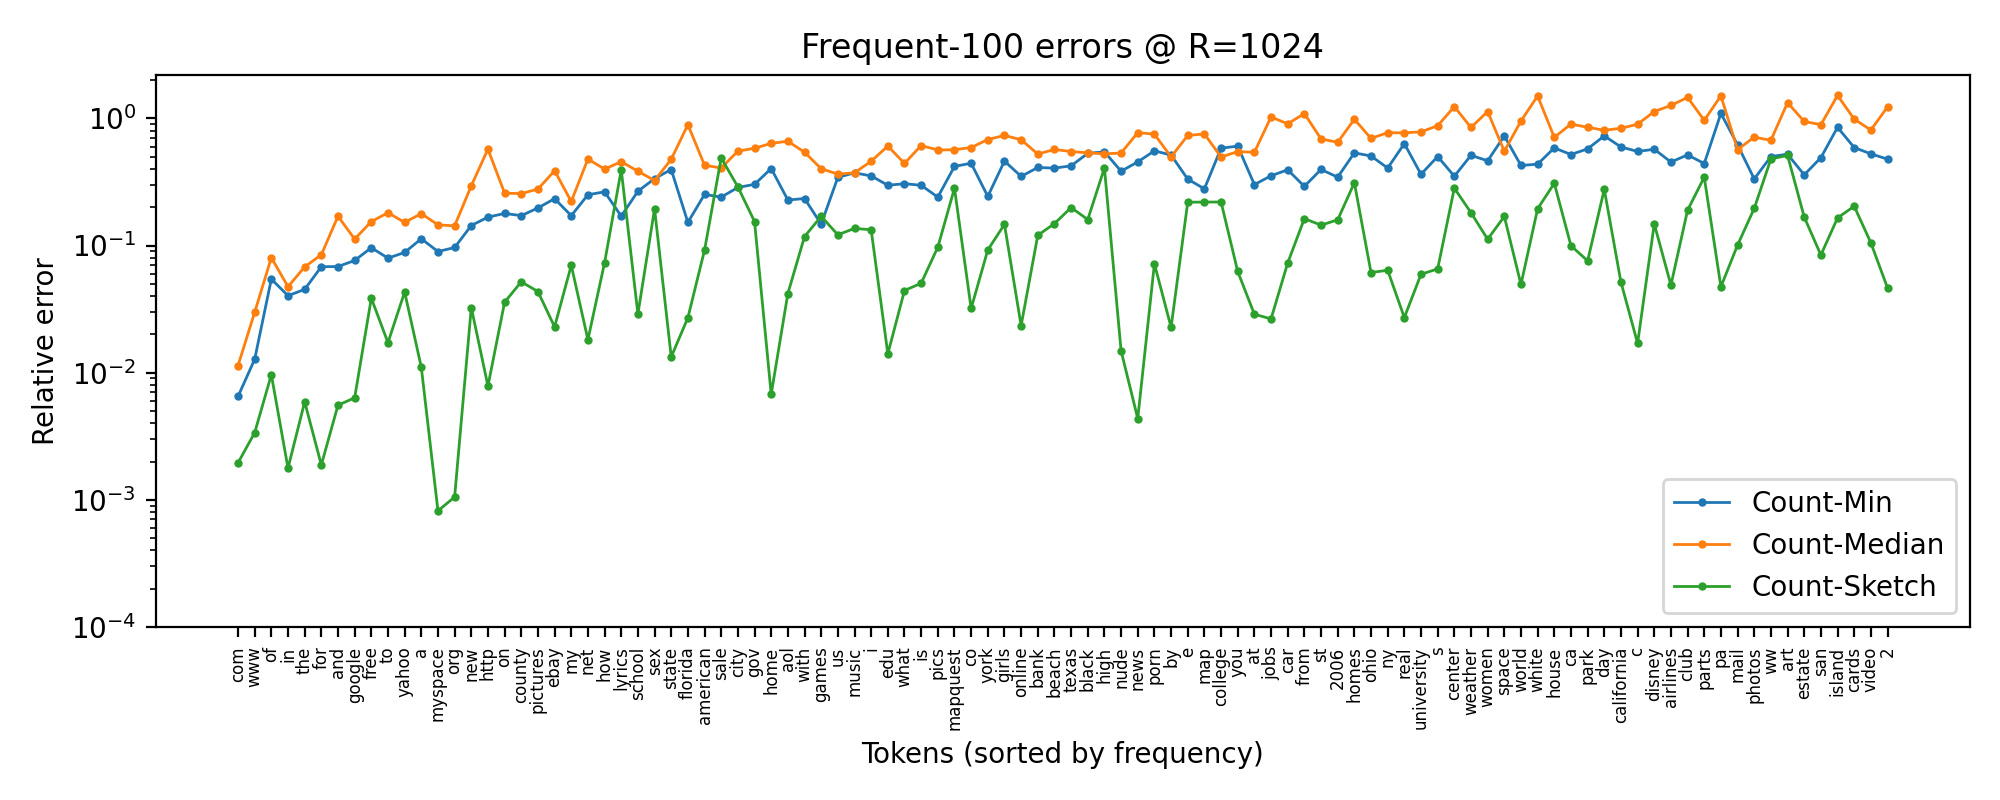
\includegraphics[width=\linewidth]{../outputs/a2/errors_R1024_Frequent_100.png}
    \caption{Frequent-100}
  \end{subfigure}\hfill
  \begin{subfigure}[t]{0.32\linewidth}
    \centering
    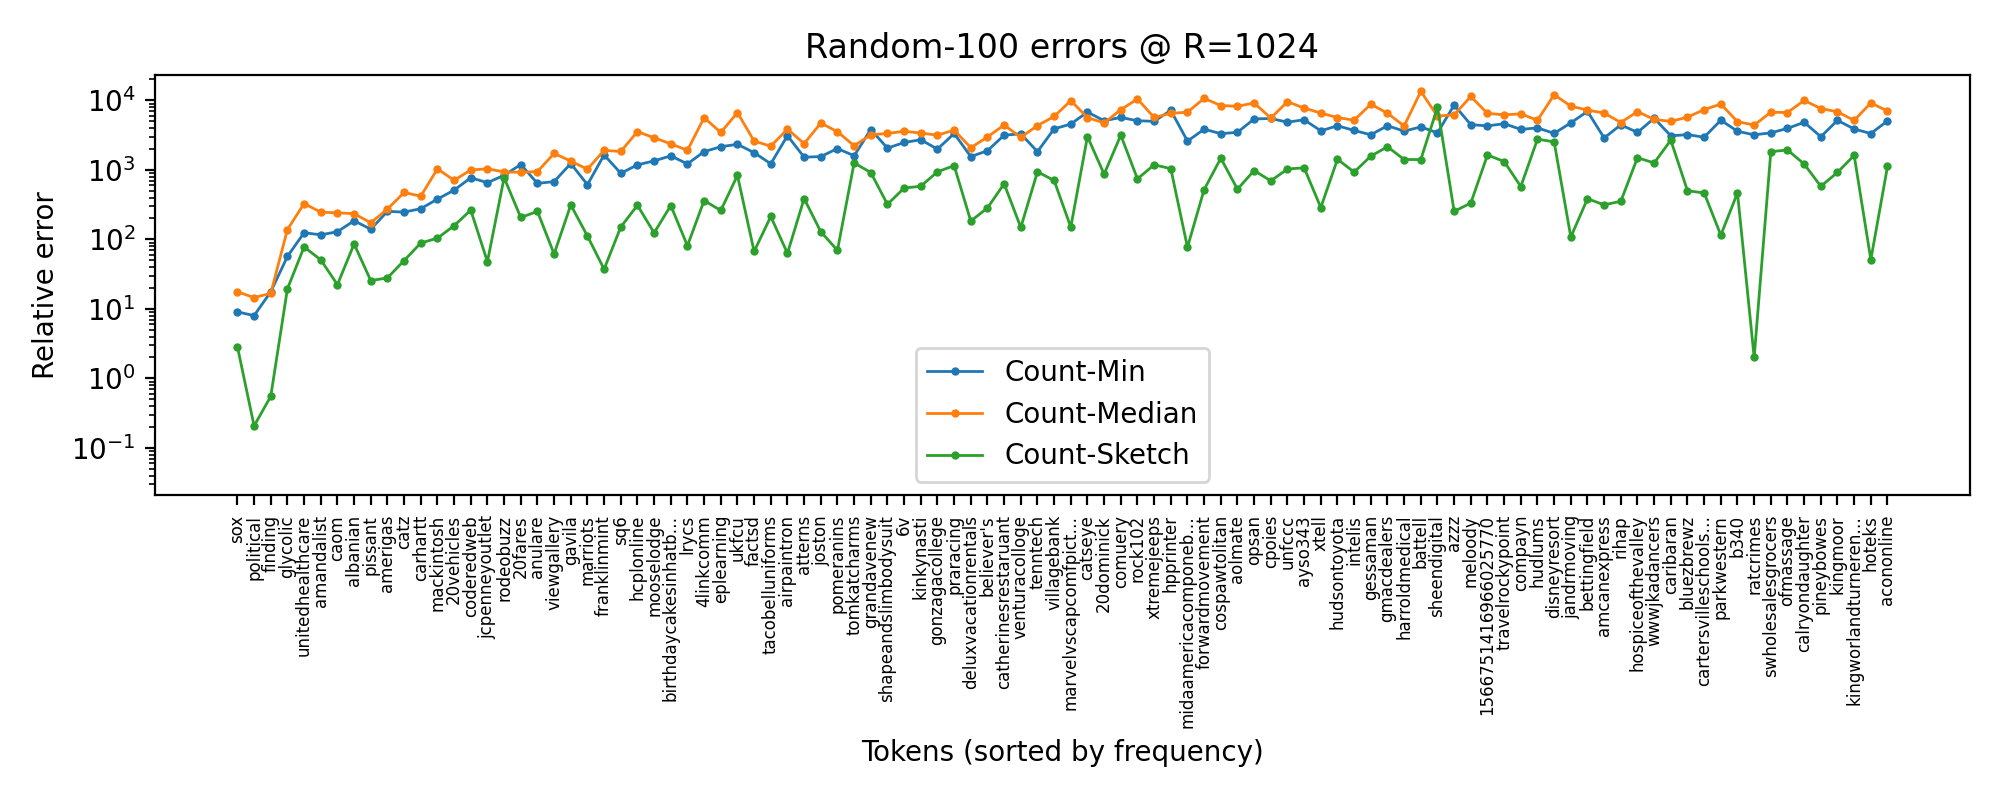
\includegraphics[width=\linewidth]{../outputs/a2/errors_R1024_Random_100.png}
    \caption{Random-100}
  \end{subfigure}\hfill
  \begin{subfigure}[t]{0.32\linewidth}
    \centering
    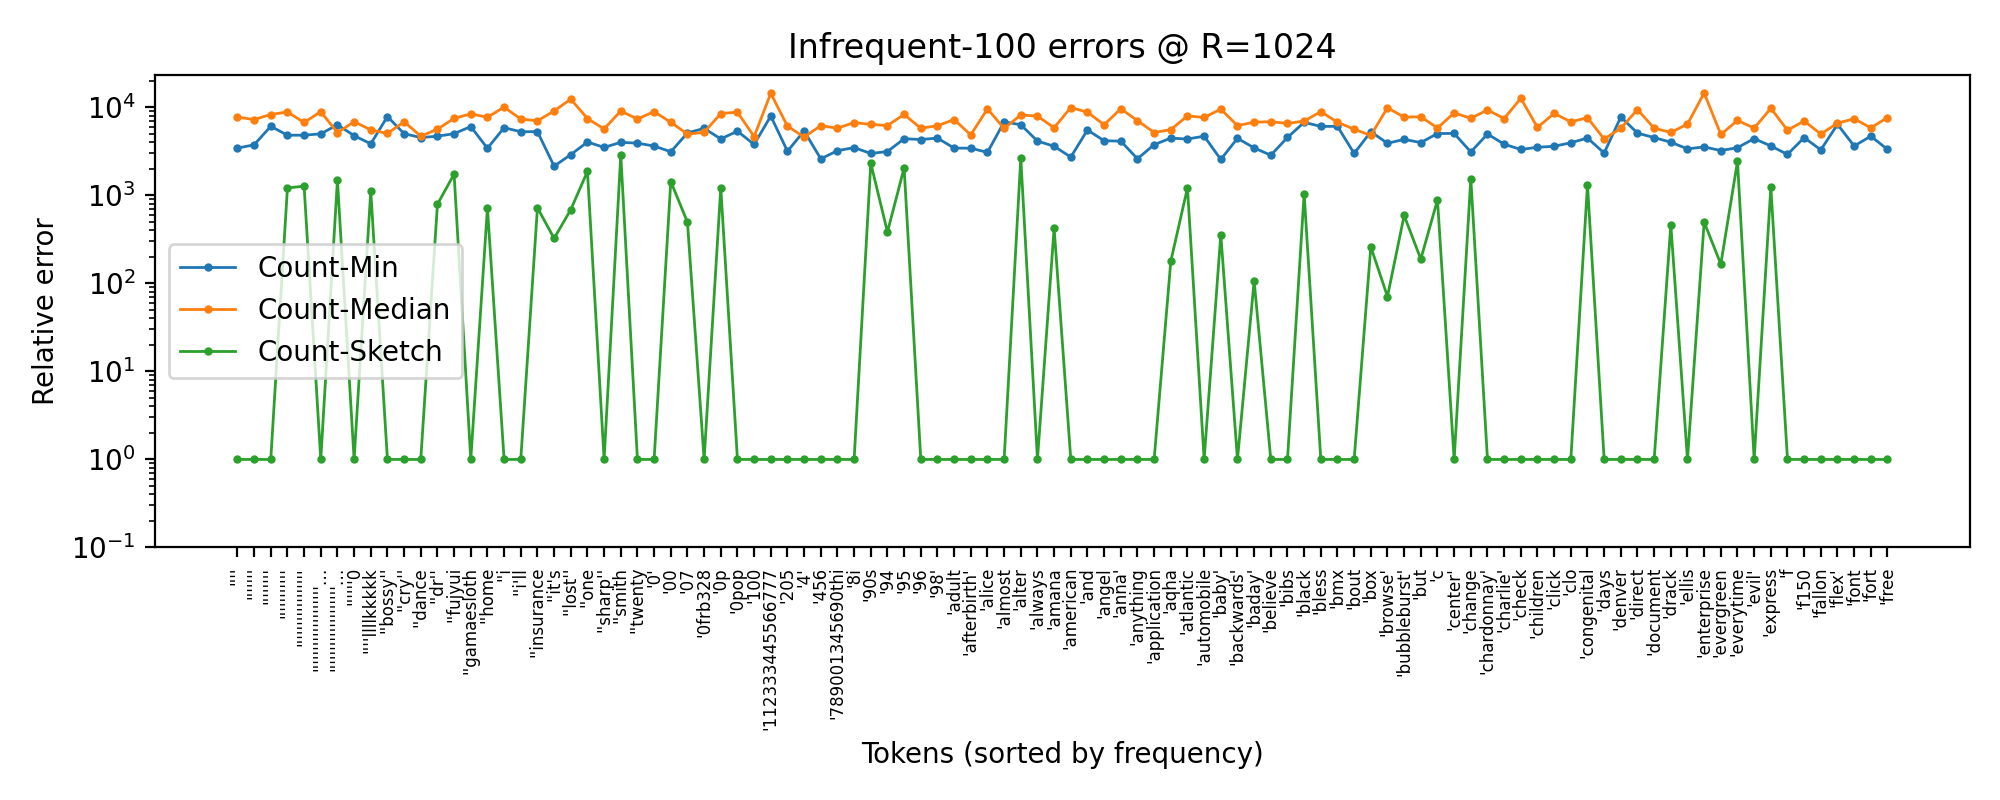
\includegraphics[width=\linewidth]{../outputs/a2/errors_R1024_Infrequent_100.png}
    \caption{Infrequent-100}
  \end{subfigure}
  \caption{Relative-error curves for $R=2^{10}$.}
  \label{fig:error-r1024}
\end{figure}

\begin{figure}[H]
  \centering
  \begin{subfigure}[t]{0.32\linewidth}
    \centering
    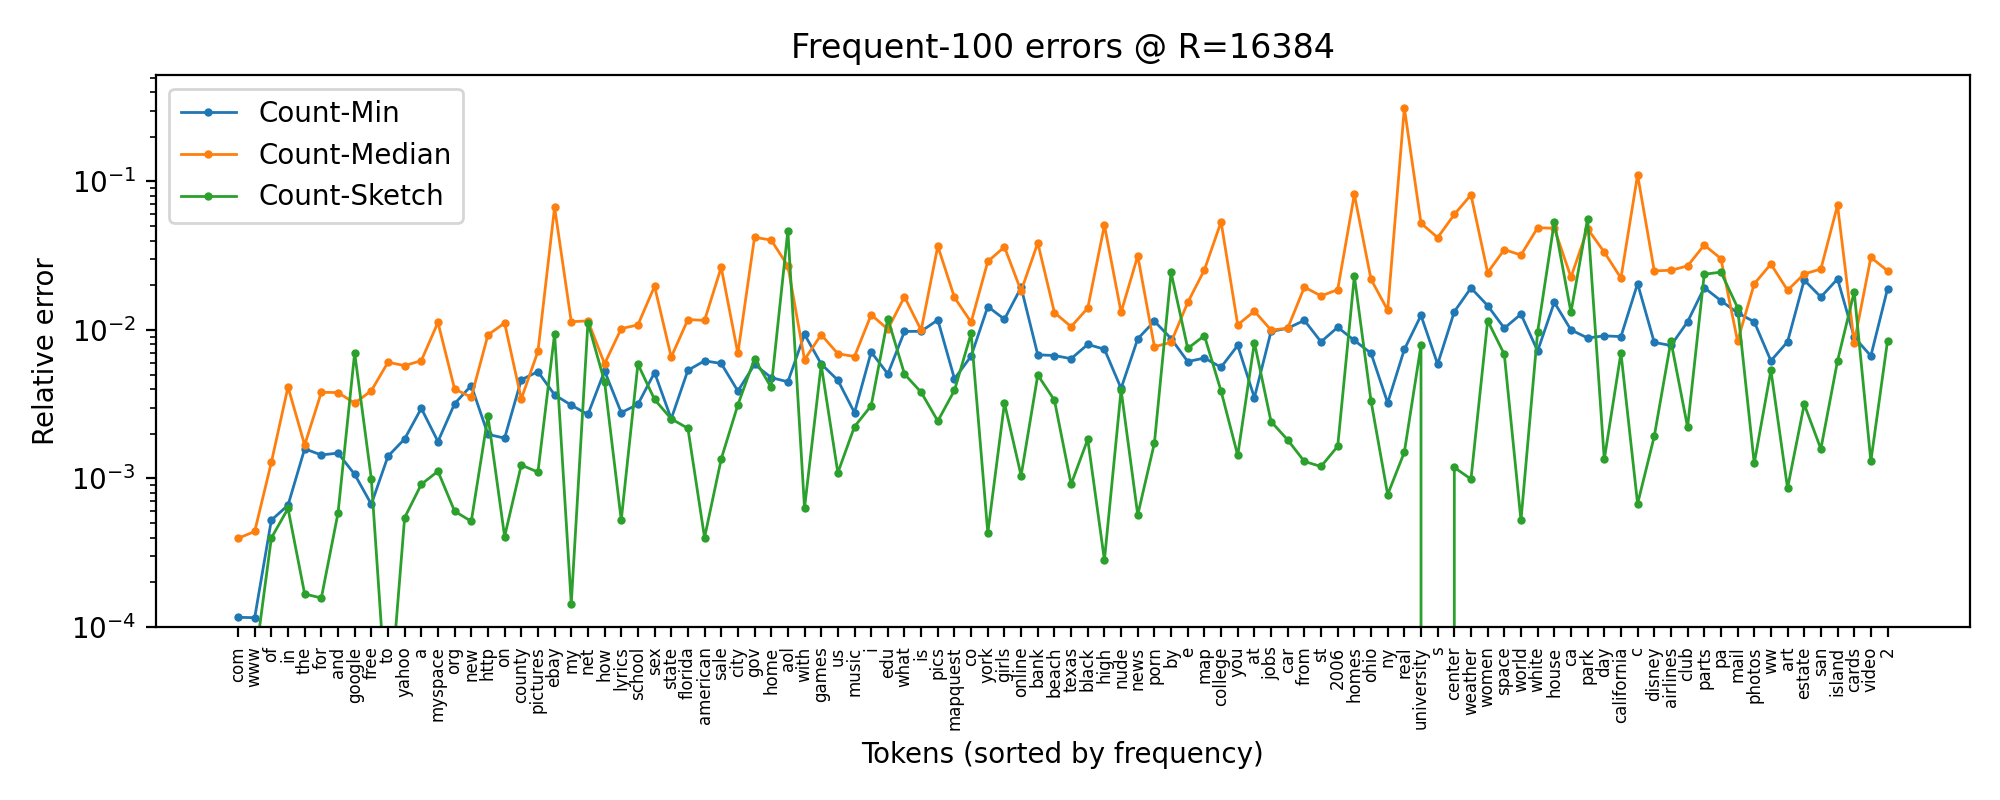
\includegraphics[width=\linewidth]{../outputs/a2/errors_R16384_Frequent_100.png}
    \caption{Frequent-100}
  \end{subfigure}\hfill
  \begin{subfigure}[t]{0.32\linewidth}
    \centering
    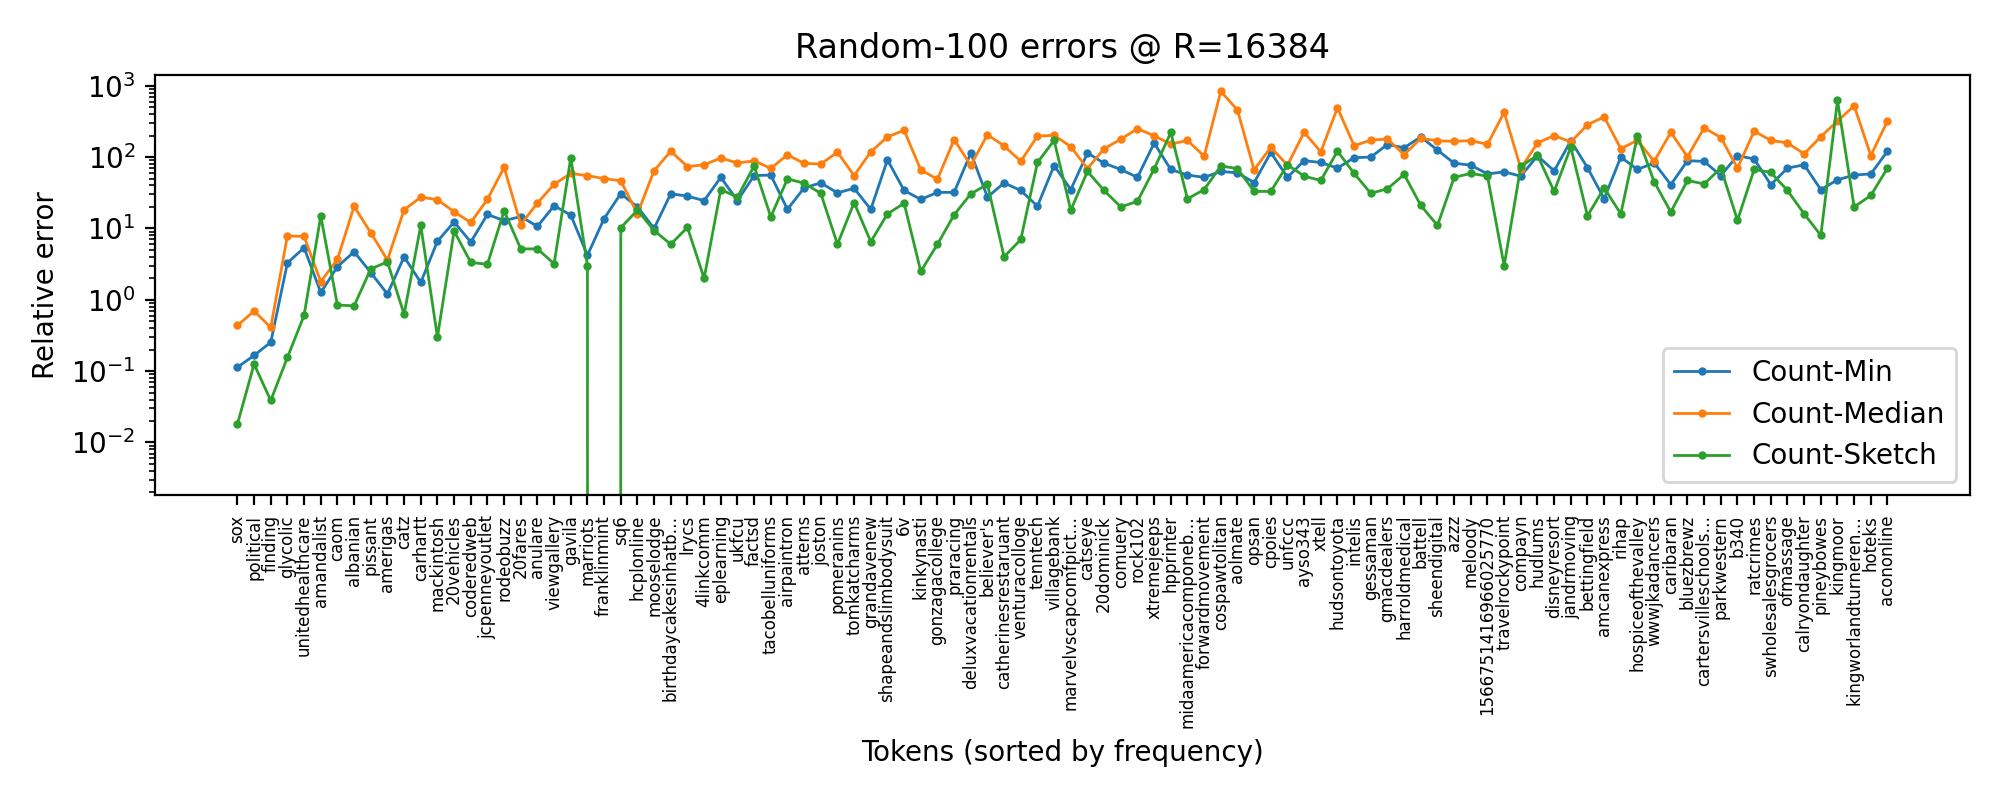
\includegraphics[width=\linewidth]{../outputs/a2/errors_R16384_Random_100.png}
    \caption{Random-100}
  \end{subfigure}\hfill
  \begin{subfigure}[t]{0.32\linewidth}
    \centering
    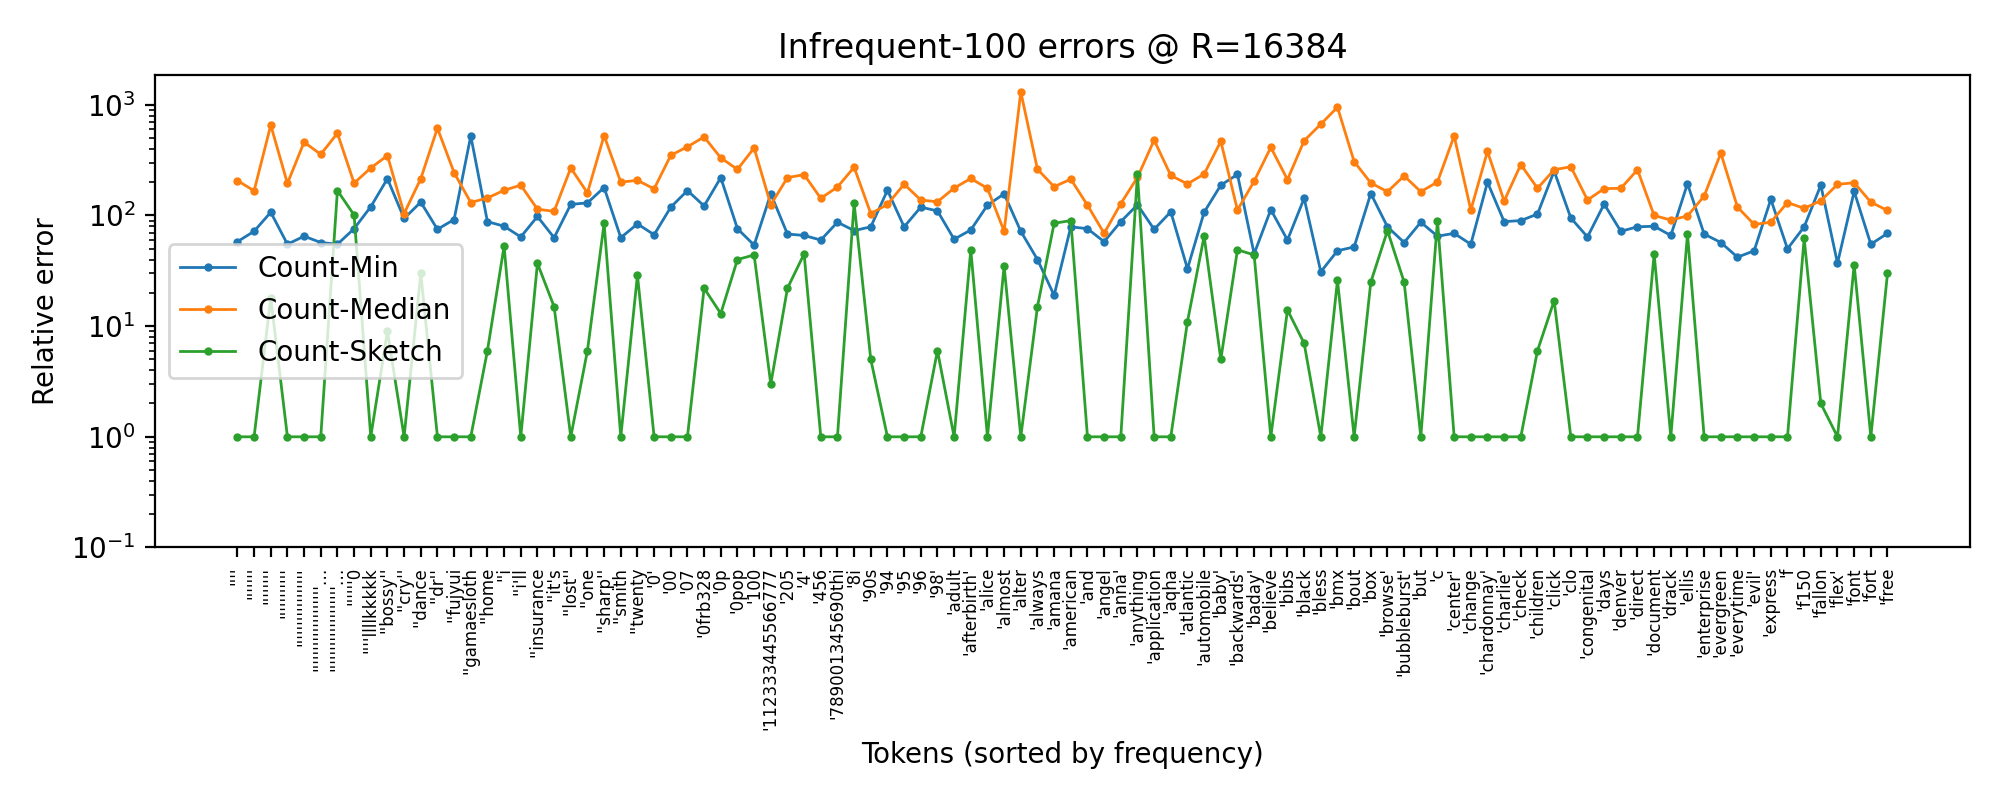
\includegraphics[width=\linewidth]{../outputs/a2/errors_R16384_Infrequent_100.png}
    \caption{Infrequent-100}
  \end{subfigure}
  \caption{Relative-error curves for $R=2^{14}$.}
  \label{fig:error-r16384}
\end{figure}

\begin{figure}[H]
  \centering
  \begin{subfigure}[t]{0.32\linewidth}
    \centering
    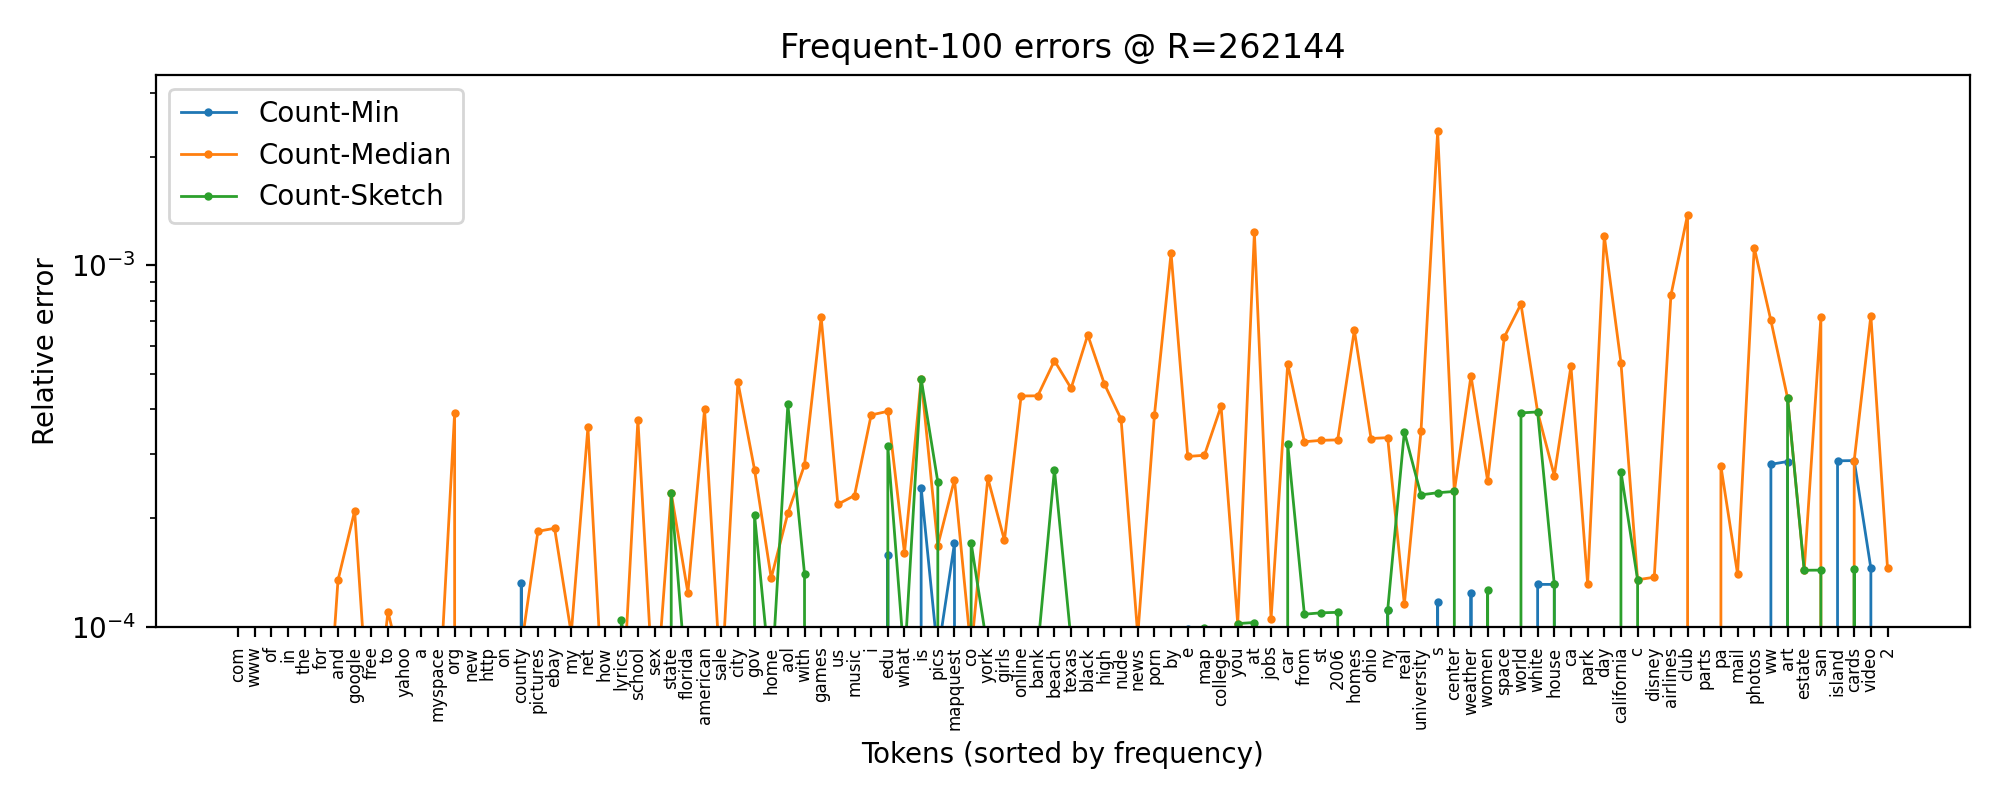
\includegraphics[width=\linewidth]{../outputs/a2/errors_R262144_Frequent_100.png}
    \caption{Frequent-100}
  \end{subfigure}\hfill
  \begin{subfigure}[t]{0.32\linewidth}
    \centering
    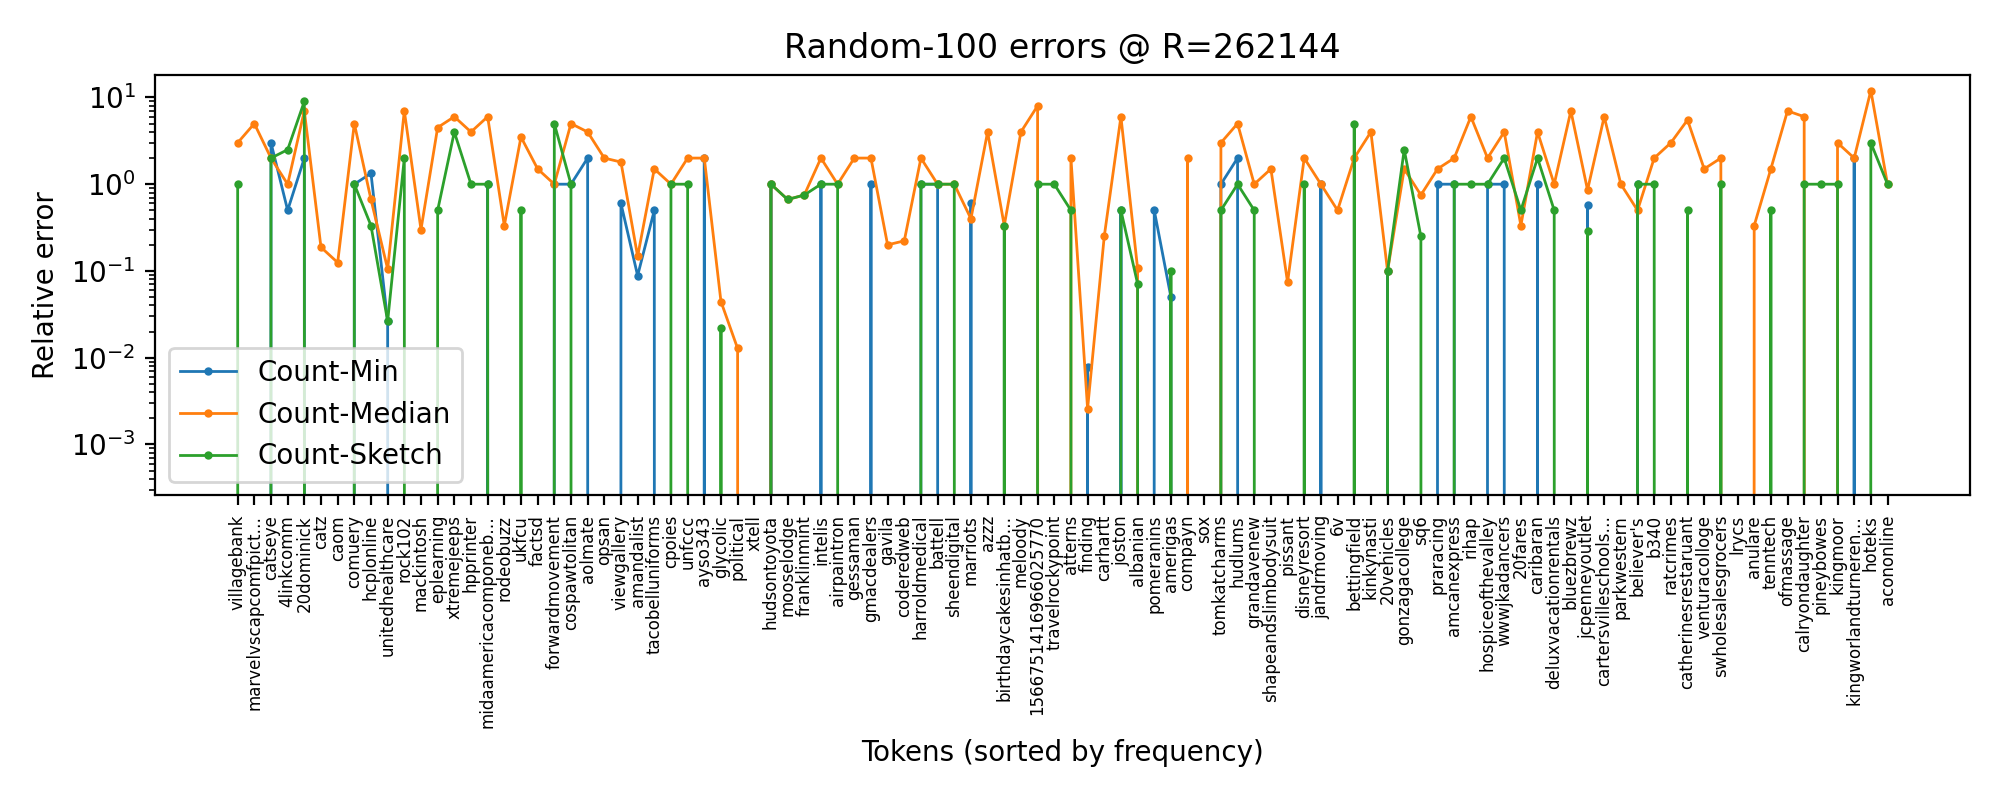
\includegraphics[width=\linewidth]{../outputs/a2/errors_R262144_Random_100.png}
    \caption{Random-100}
  \end{subfigure}\hfill
  \begin{subfigure}[t]{0.32\linewidth}
    \centering
    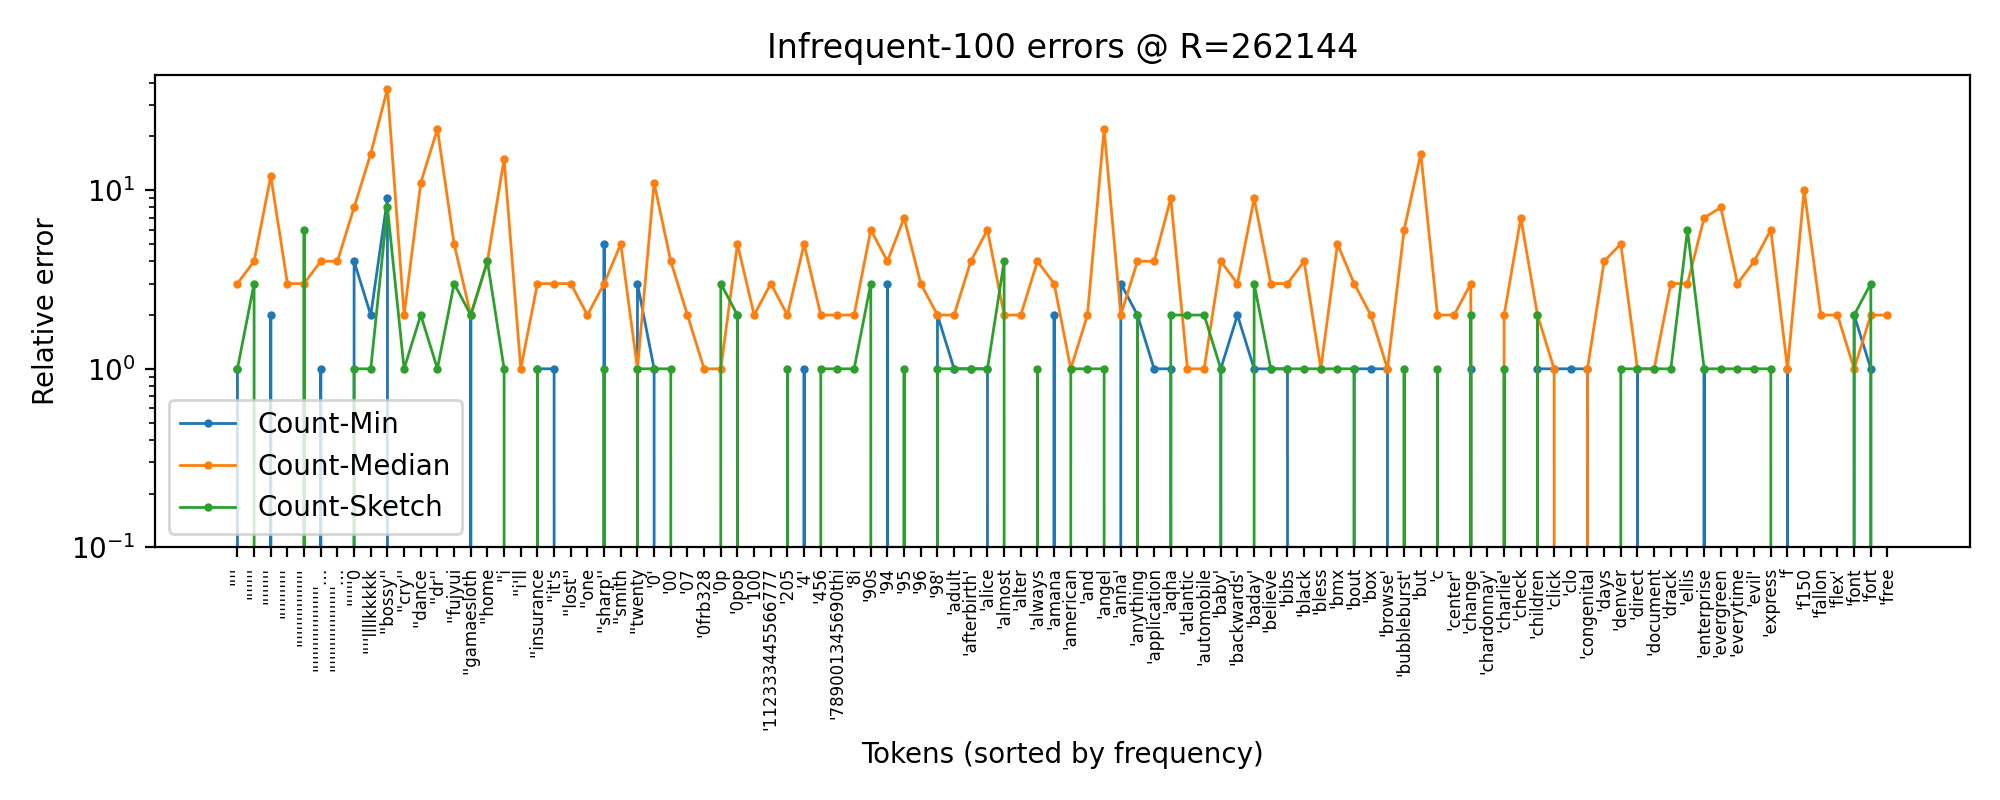
\includegraphics[width=\linewidth]{../outputs/a2/errors_R262144_Infrequent_100.png}
    \caption{Infrequent-100}
  \end{subfigure}
  \caption{Relative-error curves for $R=2^{18}$.}
  \label{fig:error-r262144}
\end{figure}

\begin{figure}[H]
  \centering
  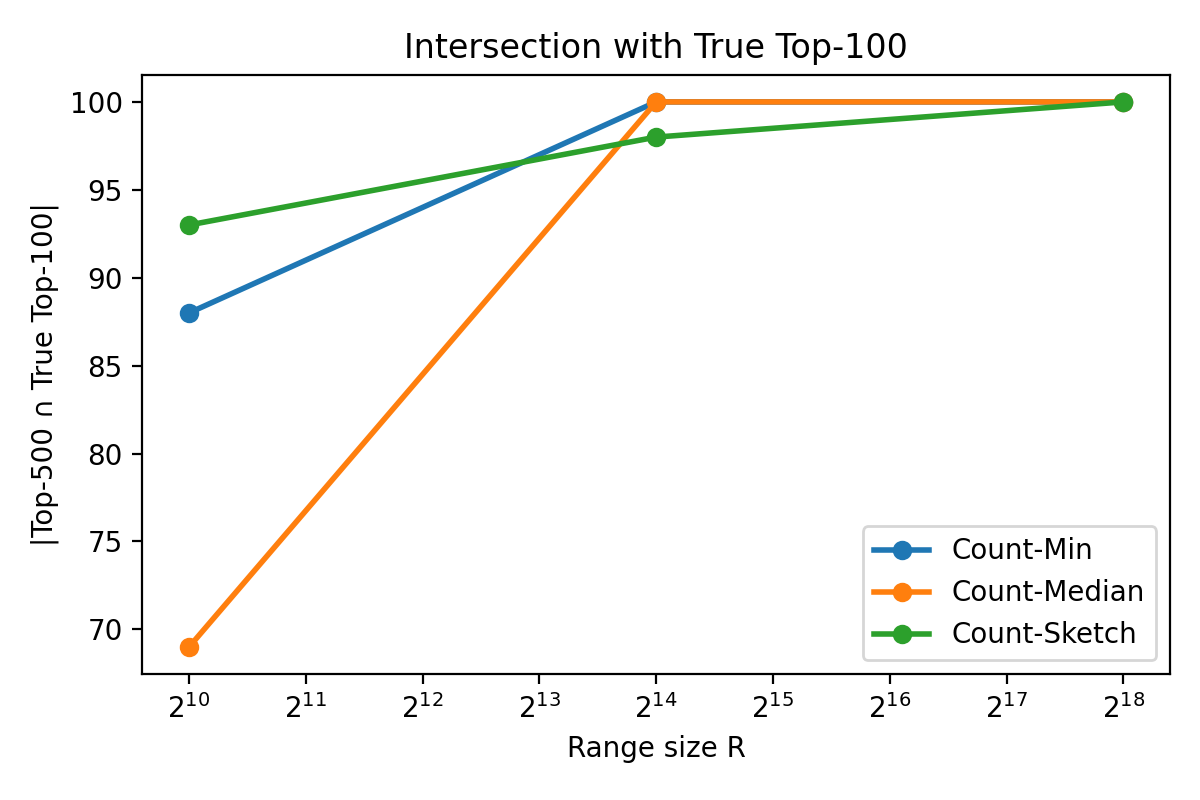
\includegraphics[width=0.55\linewidth]{../outputs/a2/top500_intersection.png}
  \caption{Intersection size of sketch top-500 with true top-100 across $R$.}
  \label{fig:top500}
\end{figure}

\subsection*{Observations for $R=2^{10}$}
\begin{itemize}
  \item Frequent tokens: Count-Min typically yields the smallest medians; Count-Median shows more spread; Count-Sketch is competitive due to signed updates.
  \item Random/Infrequent tokens: unsigned counters overestimate more often; Count-Sketch reduces these spikes via cancellation.
\end{itemize}

\subsection*{Observations for $R=2^{14}$}
\begin{itemize}
  \item Medians shrink markedly across all sketches; rare-token tails tighten compared to $R=2^{10}$.
  \item Count-Min and Count-Sketch traces flatten substantially; Count-Median retains occasional outliers on rare tokens.
\end{itemize}

\subsection*{Observations for $R=2^{18}$}
\begin{itemize}
  \item Curves are nearly flat with medians at (or near) zero for all buckets.
  \item Remaining deviations are consistent with the few residual collisions; Count-Sketch spikes are smallest.
\end{itemize}

\section{Conclusion}
The pipeline satisfies the deliverables: single-pass streaming, exact dictionary for evaluation, $d{=}5$ and $R\in\{2^{10},2^{14},2^{18}\}$, nine error plots with observations, and a top-500 intersection plot. Count-Min is biased high but improves with width; Count-Median is unbiased with higher variance on sparse items; Count-Sketch balances both via signed updates. The dictionary's space usage is recorded and noted alongside these results.

\end{document}
